\documentclass[a4paper]{article}
 
\usepackage{amsmath}
\usepackage{graphicx}
\usepackage{caption}
\DeclareCaptionFont{white}{\color{white}}
\DeclareCaptionFormat{listing}{\colorbox{gray}{\parbox{\textwidth}{#1#2#3}}}
\captionsetup[lstlisting]{format=listing,labelfont=white,textfont=white}



\usepackage{subfigure}
\usepackage{epstopdf}
\usepackage[ansinew]{inputenc}
\usepackage{listings}
\usepackage{xcolor}
%\setlength{\oddsidemargin}{0cm}
%\setlength{\evensidemargin}{0cm}
%\setlength{\topmargin}{0cm}

\usepackage[]{algorithm2e}

\usepackage{a4wide}

\title{ Simulating the mouse brain model constructed from Allen Institute for Brain Science data on the Blue Brain 4 supercomputer }
\author{Till Schumann}
%\date{}

\begin{document}
   \maketitle

\section{Introduction}
In 2014, the Neurorobotics team of the Blue Brain Project (BBP), project of the Ecole Federale Polytechnique Federale de Lausanne (EPFL), successfully produced a point-neuron model
of a mouse brain from data provided by the Allen Institute for Brain Science (Provide reference of Allen Institute).
Using NEST software, the BBP Neurorobotics team was then able to simulate a
scaled-down model of the mouse brain on a laptop computer, paving the way towards
making a mouse brain interact with an environment. A full-scale implementation of
the mouse brain model is possible, but requires the of large scale resources with low latency requirements only modern supercomputers can today provide.
The current functionality of NEST supports  generating large neuronal networks
on a super computer based an random distributions but not yet from experimental data contained in brain atlases. 
We suggest as part of this thesis to first develop the means to fully model a mouse brain from experimental data using NEST software on available supercomputing architectures.
\newpage

\subsection{Brain Simulations}
	\begin{itemize}
      \item Short introduction to neuroscience 
      \item Short overview over simulators: NEST, NEURON, STEPS
      \item Possibilities/limits of simulations
   \end{itemize}
   
\subsection{Virtual mouse}
	\begin{itemize}
      \item Available data
      \item Why of interest
   	\end{itemize}   

\subsection{Allen Brain Atlas}
   Allen Institute for Brain Science provides a high-resolution map of neural connections in the mouse brain.
   It contains several injection experiments. The provided datasets of the experiments 
   contain a 3D image of the injection and a 3D image of its axonal projection labeled by viral
   tracers.
   
   \begin{figure}[ht!]
   	\begin{center}
        \subfigure[Injection sites - showing all available experiments]{%
            \label{fig:allInjections}
            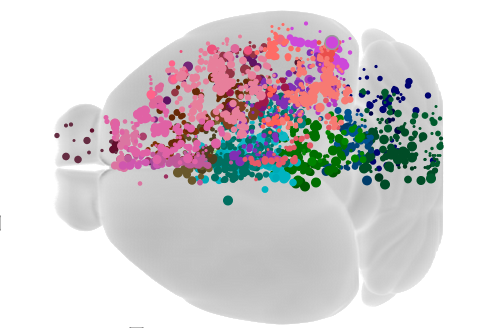
\includegraphics[width=0.4\textwidth]{../connectionBrowser_allinjections.png}
        }
        \hspace{1cm}
        \subfigure[Projection density of one experiment]{%
            \label{fig:oneProjection}
            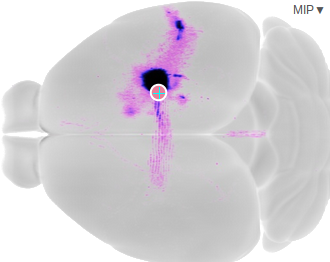
\includegraphics[width=0.32\textwidth]{../connectionBrowser_oneinjections.png}
       }
    	   \end{center}
    	\caption{%
        The pictures are inverted and copied from the Allen Brain Atlas.
     }%
   \label{fig:atlas}
   \end{figure}
   
\subsection{BBP recipe}
	The Blue Brain project   

\subsection{NEST}
NEST is a simulator for spiking neural network models that focuses on the dynamics, size and structure of neural systems rather than on the exact morphology of individual neurons. The development of NEST is coordinated by the NEST Initiative. NEST is ideal for networks of spiking neurons of any size, for example:
Models of information processing e.g. in the visual or auditory cortex of mammals, models of network activity dynamics, e.g. laminar cortical networks or balanced random networks and models of learning and plasticity. A NEST simulation tries to follow the logic of an electrophysiological experiment that takes place inside a computer with the difference, that the neural system to be investigated must be defined by the experimenter. The definition is based on number of neurons with parameters and connections between these neurons. NEST supports the generation based on probabilistic values. The stochastic settings of a neuronal network can be used to create its artificial copy inside of NEST. To manipulate or observe the network dynamics, the experimenter can define so-called devices which represent the various instruments (for measuring and stimulation) found in an experiment. These devices write their data either to memory or to file. 

\subsection{Visualization}
To interpret the output of a neuronal simulation the spiking activity of the neurons is analyzed, mostly. Different types of methods allow to extract stochastic characteristics from spike trains. Besides this visualization of the spike trains taking their location into account, allows to create a video, which shows the activity of the neuronal network.




\section{Analysis}

\subsection{Available resources}   
The Blue Brain 4 system is a set of tightly integrated high-performance resources. It is comprised of a four-rack IBM BlueGene/Q system 65 536 PowerPC A2 1.6 GHz cores for computing, providing a peak performance of 839 TFlops 65 TB of RAM, a shared parallel filesystem based on GPFS / GSS of a capacity in excess of 4 petabytes and a bandwidth exceeding 40GB/s A FDR Infiniband network Job scheduling across the system's components is performed by Slurm. 

\subsection{NEST simulations}
The standard use-case for the NEST simulator is a stochastic-driven simulation. This means
that the circuit is characterized by stochastic parameters (e.g. number of synapses between neurons).
The circuit is build-up inside of NEST using only these parameters.
This means that the amount of need data is small. It allows to build-up large scale simulation
with a few arguments.

\subsection{Memory consumption of NEST}
The memory usage of the newest NEST release 2.6.0 can be calculated with following equation. \cite{kunkel2014spiking}
\begin{equation}
  \Pi(M,T,N,K) =  \Pi_0 + \Pi_n(M,N)  + \Pi_c(M,T,N,K)
  \label{eq:NESTmemconsumption}
\end{equation} 
\begin{equation}
  \Pi_n(M,N) = N_M*1100
\end{equation}
\begin{equation}
  \Pi_c(M,T,N,K) = 0.33 * T * N + T * N^1_c * 24 + T*(N-N^1_c)*128 + N_M*K*52
\end{equation}
$\Pi$ is the memory consumption. $\Pi_0$ is the initial memory consumption of NEST.
For the \emph{JUQUEEN} its around 26 MB and for \emph{K} around 260 MB.
$M$,$T$, $N$, $K$ correspond to number of MPI Nodes, number of threads per node, number of neurons and number of outgoing connection per neuron.
For the calculation there are some simplifications done.
The model uses the \emph{iaf\_psc\_alpha} neuron model for all neurons. There are only static synapses.
The number of incoming connection per neuron $K$ is not known. Only the number of outgoing connections is known.
To get some results anyway, it is expected that they are similar.
Furthermore the term of expected number of neurons without any VP-local target is set to zero, which is the worst case for the consumption of memory.

\subsection{Interfaces}
\subsection{Circuit generation}
\begin{itemize}
      \item Create point circuit from available data
      \item Fuse data from the Allen Brain Atlas and the BBP recipe
   \end{itemize}

\subsubsection{Long range connections}
A set of experiments is used to connect neurons located at the injections
to the neurons at the projections. Unfortunately all injections from these experiments do not
cover the whole brain. So there are neurons which are not injected
by any experiment. Therefore all neurons which are not injected should use the projection
from the nearest injection. To map pixels of the 3D pictures to neurons, the neurons are assigned to voxels, which represent the pixels. In a first step the best experiment is chosen for each voxel based on the minimal total injection per experiment. In the second step all voxels in the right hemisphere, which have not received an experiment take the experiment from the nearest voxel, which has an experiment. In the third step the given experiments are used to generate the connections for the related neurons. To get connection for the both hemispheres the information is mirrored along the z-axis.

\begin{figure}[ht!]
   	\begin{center}
        \subfigure[Illustration injection]{%
            \label{fig:allInjections}
            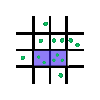
\includegraphics[width=0.15\textwidth]{cg_illustration_injection.eps}
        }
        \hspace{0.5cm}
        \subfigure[Illustration projection]{%
            \label{fig:oneProjection}
            
\includegraphics[width=0.15\textwidth]{cg_illustration_projection.eps}
       }
       \hspace{0.5cm}
       \subfigure[Merge experiment]{%
            \label{fig:allInjections}
            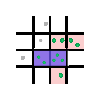
\includegraphics[width=0.15\textwidth]{cg_illustration_merge.eps}
        }
        \hspace{0.5cm}
        \subfigure[specify source and target neurons]{%
            \label{fig:oneProjection}
            
\includegraphics[width=0.15\textwidth]{cg_illustration_neurons.eps}
       }
    \end{center}
    	\caption{%
        Assign density of experiments to neurons.
     }%
   \label{fig:atlas}
   \end{figure}
   
   \begin{itemize}
      \item Implementation
      \item Parallel efficiency, memory consumption and limits
   \end{itemize}
   
\subsubsection{Short range connections}
The Blue Brain Project has investigated over the last years in experiential work the relation of different synapse types.
They collected their findings in a recipe which allows to get the synapse type for different neuron types.
The neuron types depend on their layer, electrical and morphological type. The recipe defines which synapses are between 
which kind of neurons. The generated synapses connect neurons to its neighborhood. The neighborhood is defined as a
column in the same orientation as the neuron has.


\begin{figure}[ht!]
   	\begin{center}
        \subfigure[contain all neuron information]{%
            \label{fig:shortColumn}
            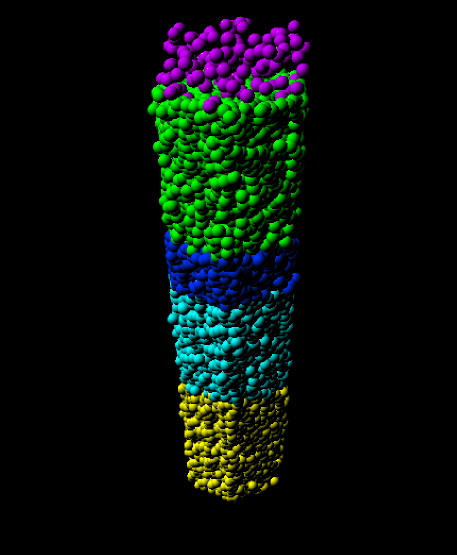
\includegraphics[width=0.3\textwidth]{../shortrange/g3111.png}
        }
        \hspace{1cm}
        \subfigure[contain all synapse information]{%
            \label{fig:shortColumnInCircuit}
            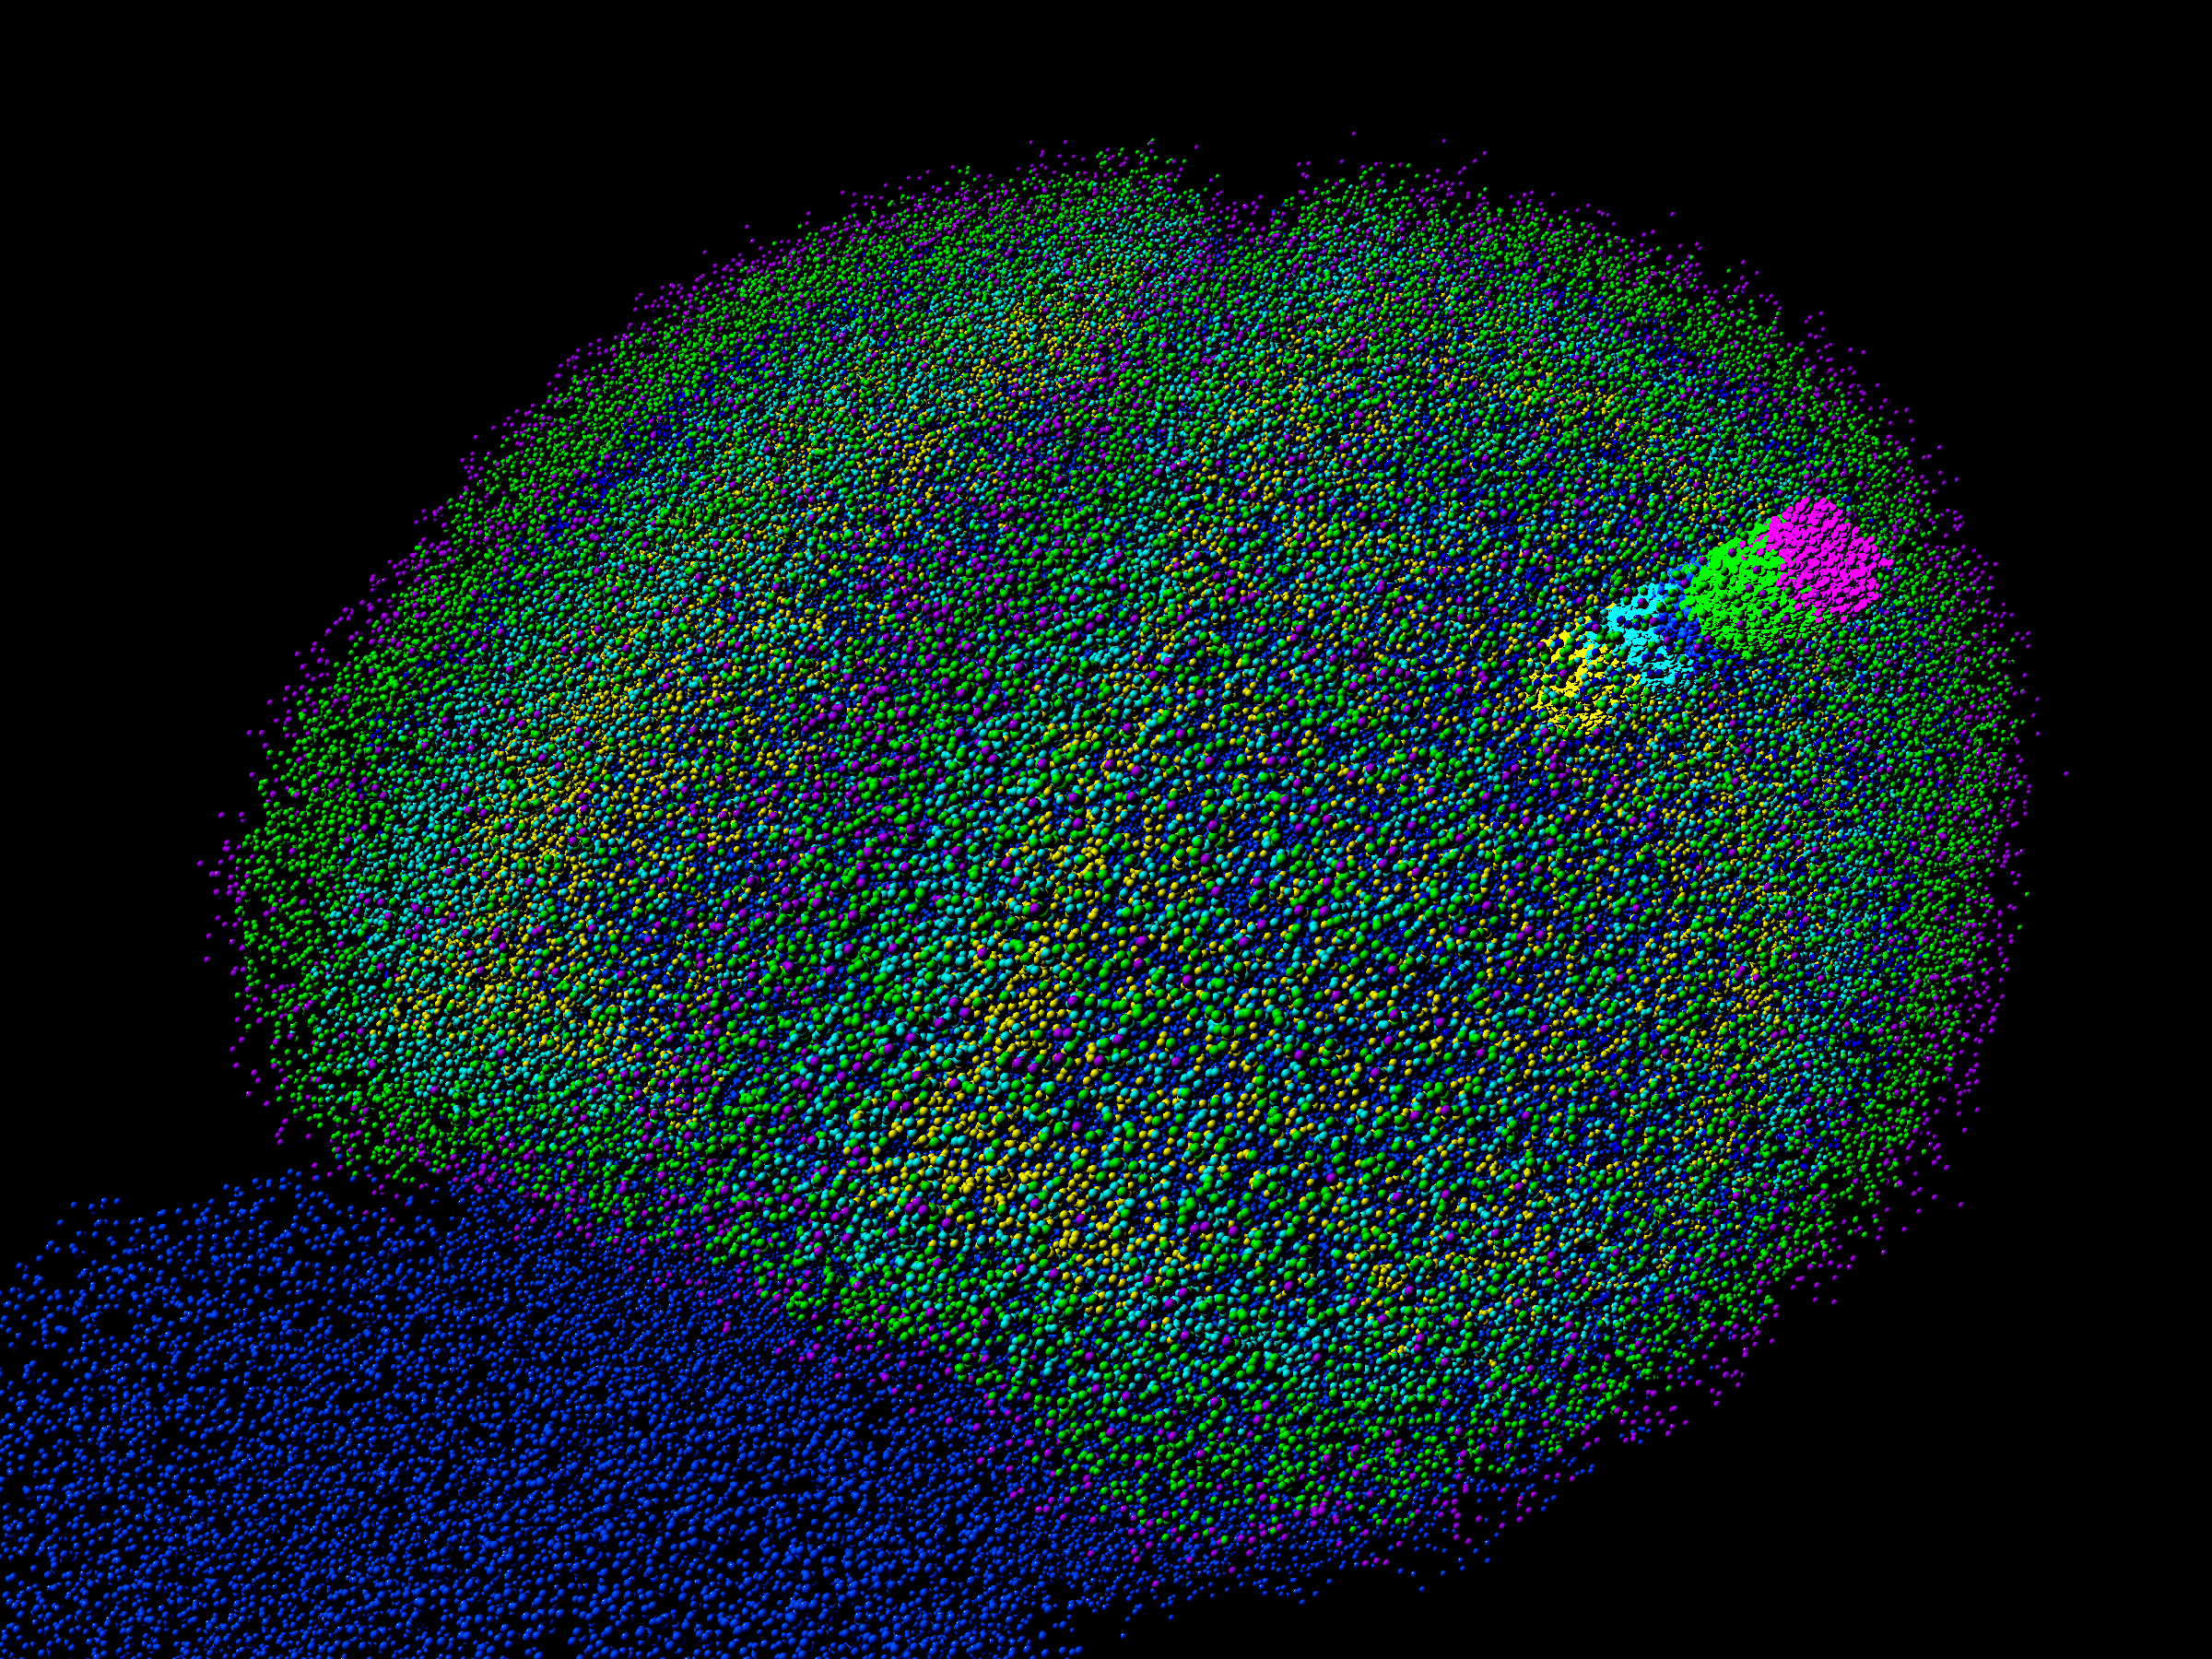
\includegraphics[width=0.485\textwidth]{../shortrange/column_in_brain_4_edit.png}
       }
    	   \end{center}
    	\caption{%
        3D visualization of the original Blue Brain Project column (left) and the reconstructed mouse
isocortical column that has a similar neuron density (right). Layers 1, 2/3, 4, 5 and 6 are
shown in different colors.
     }%
   \label{fig:atlas}
   \end{figure}

\begin{itemize}
      \item Implementation
      \item Parallel efficiency, memory consumption and limits
   \end{itemize}

\subsection{Data-driven simulation}
As we generated the circuit in a preprocessing step. Neuron and point to point synapse information are given.
Thus we call it a data-driven simulation. We do not use the build-up functionality from NEST.
Hence we have to load the whole circuit from file.

\subsection{Parallel IO}
Build-up a large scale neuronal network from point to point connectivity results in new requirements for data processing and the data format. The parallel IO is strictly limited by the given bandwidth. Clumsy parallel IO access can even lower the resulting bandwidth.
Thus the distribution of the parallel loading has to be carefully chosen. HDF5 allows parallel access to the same file.

\subsection{Pipeline}
The requirements for all implementations are the usability for the scientists. Besides efficient implementation the users should be able to manipulate the data on different levels. Creating one simulation from data based on the Allen Brain Institute is not the main goal of this thesis. In fact the implementations should complete the tool chain to run data-driven simulations with NEST and visualize them, based on Allen injection experiments. Therefore the proposed pipeline contains data formats which can be manipulated. Processing the needed amount of data takes time and has to be executed on large compute clusters. Thus an interactive usage of the tools is not reasonable.

\section{Implementation}

\subsection{Data format}

\begin{figure}[ht!]
   	\begin{center}
        \subfigure[contain all neuron information]{%
            \label{fig:allInjections}
            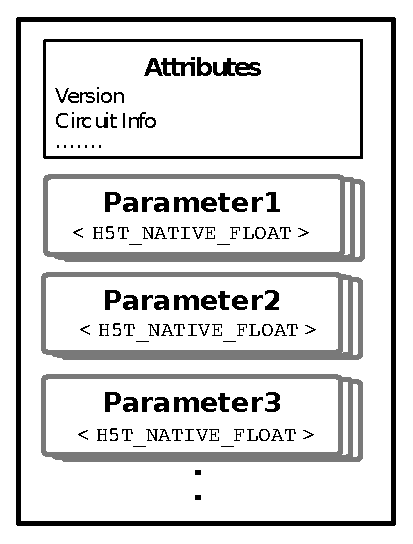
\includegraphics[scale=0.5]{hdf5_neuron_format.eps}
        }
        \hspace{1cm}
        \subfigure[contain all synapse information]{%
            \label{fig:oneProjection}
            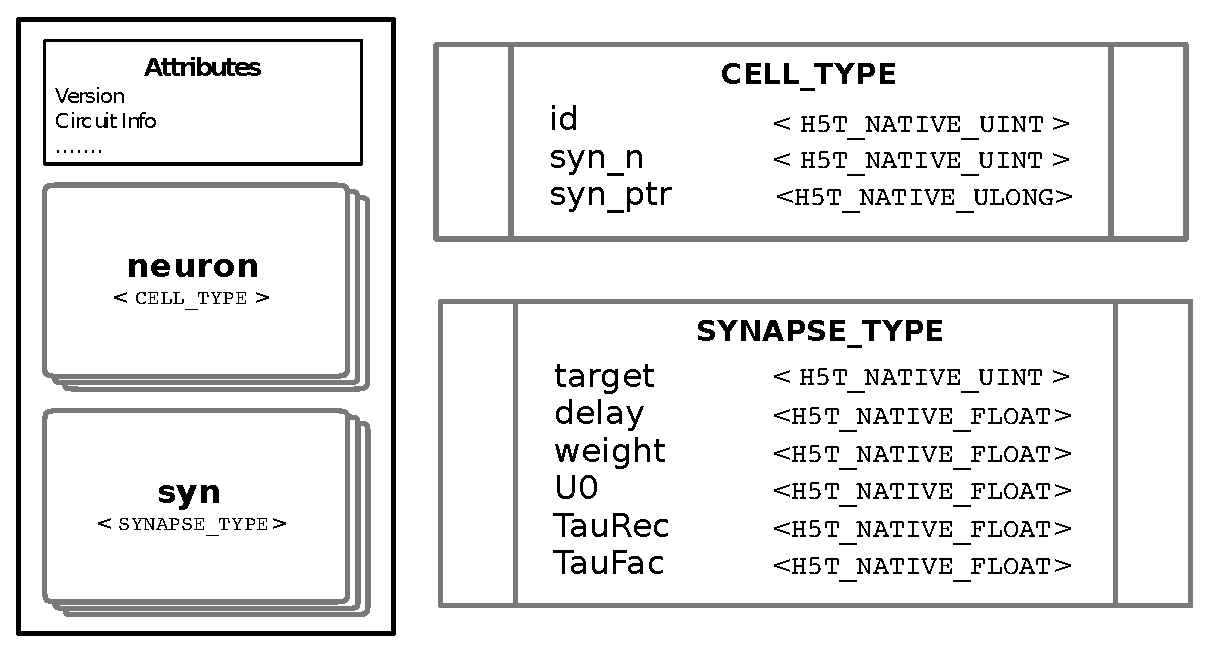
\includegraphics[scale=0.41]{hdf5_syn_format.eps}
       }
    	   \end{center}
    	\caption{%
        The HDF5 file formats.
     }%
   \label{fig:atlas}
   \end{figure}

\begin{itemize}
      \item Synapse data format
      \item Neuron data format
\end{itemize}

\subsection{Circuit generation}
Rewriting the sequential python script to a hybrid C++ application require a parallel implementation of a parallelization strategy and the usage of 
a parallel random generator. For the parallelization strategy a Master-Slave approach is chosen to distribute the workload dynamically on the nodes.
Communication between the individual nodes is not necessary. Only the workload management is handled by the master node.
For the random generator Random123 is used, because it has good performance and it is easy to use.
It ensures reproducible results without correlations in the generated values. 


\begin{itemize}
      \item Connection properties affect memory balance
      \item Balance neurons on nodes to achieve better memory balance
\end{itemize}

\subsection{Circuit validation}
\begin{itemize}
      \item Visual validation of synapses
      \item Visual validation of spiking activity
      \item Statistical properties are not analyzed in this work 
\end{itemize}

\begin{figure}[ht!]
\centering
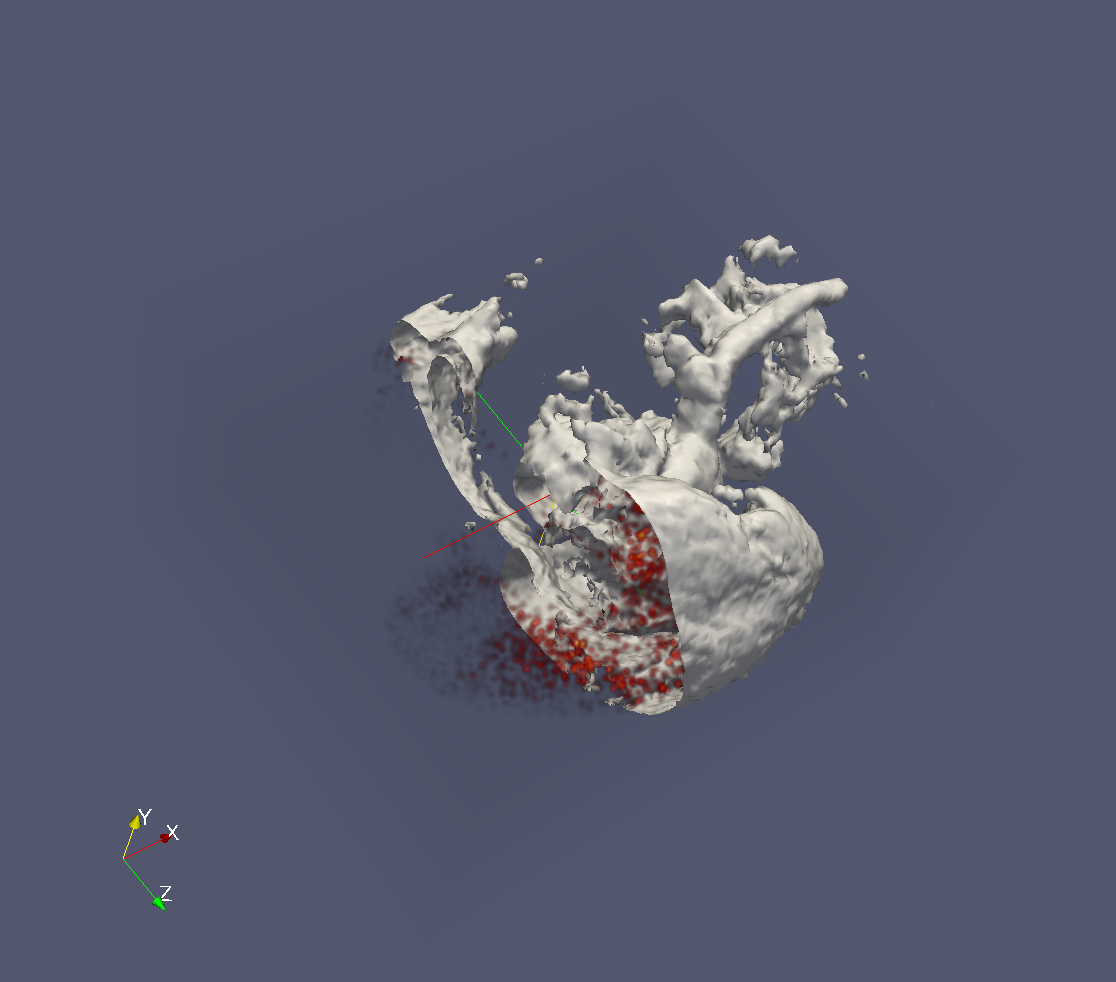
\includegraphics[width=0.4\textwidth]{paraview_ex.png}
\end{figure}

\subsection{NEST import module}

The neuronal spiking network simulator NEST is developed in \emph{C++} and delivers
an user interface based on an own description language \emph{SLI} and  and a Python interface.
The new use case shall be integrated into the standard work flow of NEST.
Besides the functionality in \emph{C++} the interfaces have to be extended.
The difficulties of the network generation is based on a difference in 
the NEST internal data structure and the data delivered by the Allen Institute.
Connection information contains target and source neurons besides biochemical
information of the synapses. Because of the in vitro injection methods the
connection information maps the synapse from the source to the target neurons.
For multi process simulations NEST distributes all neurons based on a modulo function 
to the processes. Because of memory optimizations the synapses are only stored on the
post synaptic process. This means that the connection information is stored
on the process, where the target neuron is located. Therefore a transformation of the given data is
necessary. Preprocessing of the input data should be avoided as far as possible to capture
future use cases.
The resulting implementation shall load the connection information efficiently in parallel,
distribute the synapse information to the post synaptic node and store it in
the NEST data structure.
Further requirements of the implementation are an efficient use of the available resources as
memory and computation power. 


\subsubsection{Import neurons}

\emph{H5NeuronCsX\_s\_s\_a\_s} expects 4 input parameters:
\begin{itemize}
      \item Name of the a subnet dataset (String).
The subset has to contain for each neuron an integer value.
The neurons are grouped together by this subnet value.

      \item A list of all datasets which values are interpreted as list of parameters.
      
      \item Name of the used neuron model
      
      \item path to the HDF5 file 
\end{itemize}
The function returns the neuron id of the first neuron it created.

\begin{lstlisting}[label=sliNeurons,caption=Calling the neuron import module via H5NeuronCsX\_s\_s\_a\_s SLI command ]
/neuronmodel /aeif_cond_exp def
/subnet (subnet) def
/neuronparams [(C_m) (Delta_T) (E_L) (V_reset) (V_th) (a) (b)] def
/filepath (circuit/ptneu_brain.h5) def
subnet neuronparams neuronmodel filepath H5NeuronCsX_s_s_a_s /offset Set
\end{lstlisting}



\begin{itemize}
      \item Sli command with parameters
      \item Functionality
\end{itemize}

\subsubsection{Import synapses}


\begin{figure}[ht!]
\centering
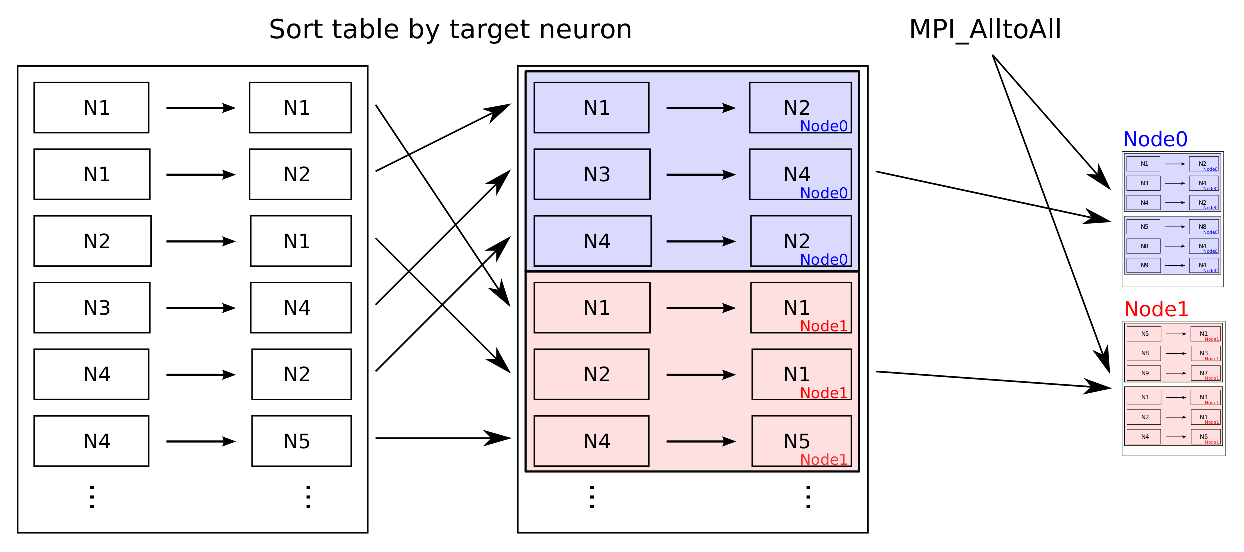
\includegraphics[scale=0.7]{sort_table_all_alltoall.eps}
\caption{Distribute synapses to the nodes.}
\end{figure}


\emph{H5SynapseTll\_i\_s\_a\_s} expects 4 input parameters:
\begin{itemize}
      \item Offset of the neuron ids. Mostly it is equal to first neuron id returned by \emph{H5NeuronCsX\_s\_s\_a\_s}

      \item A list of all columns which values are interpreted as parameters.
      
      \item Name of the used synapse model
      
      \item path to the HDF5 file 
\end{itemize}
The function returns the neuron id of the first neuron it created.

\begin{lstlisting}[label=sliSynapses,caption=Example importing synapses]
/synmodel /tsodyks2_synapse def
/synparams [(delay) (weight) (U0) (TauRec) (TauFac)] def
/filepath (circuit/syn.h5) def
offset synparams synmodel filepath H5SynapseTll_i_s_a_s
\end{lstlisting}
\begin{itemize}
      \item Sli command with parameters
      \item Functionality
      \item Explain Communication
      \item customizable
\end{itemize}

\subsection{Analysis of simulation results}


\section{Discussion}
\subsection{Circuit properties}

\begin{figure}[ht!]
\centering
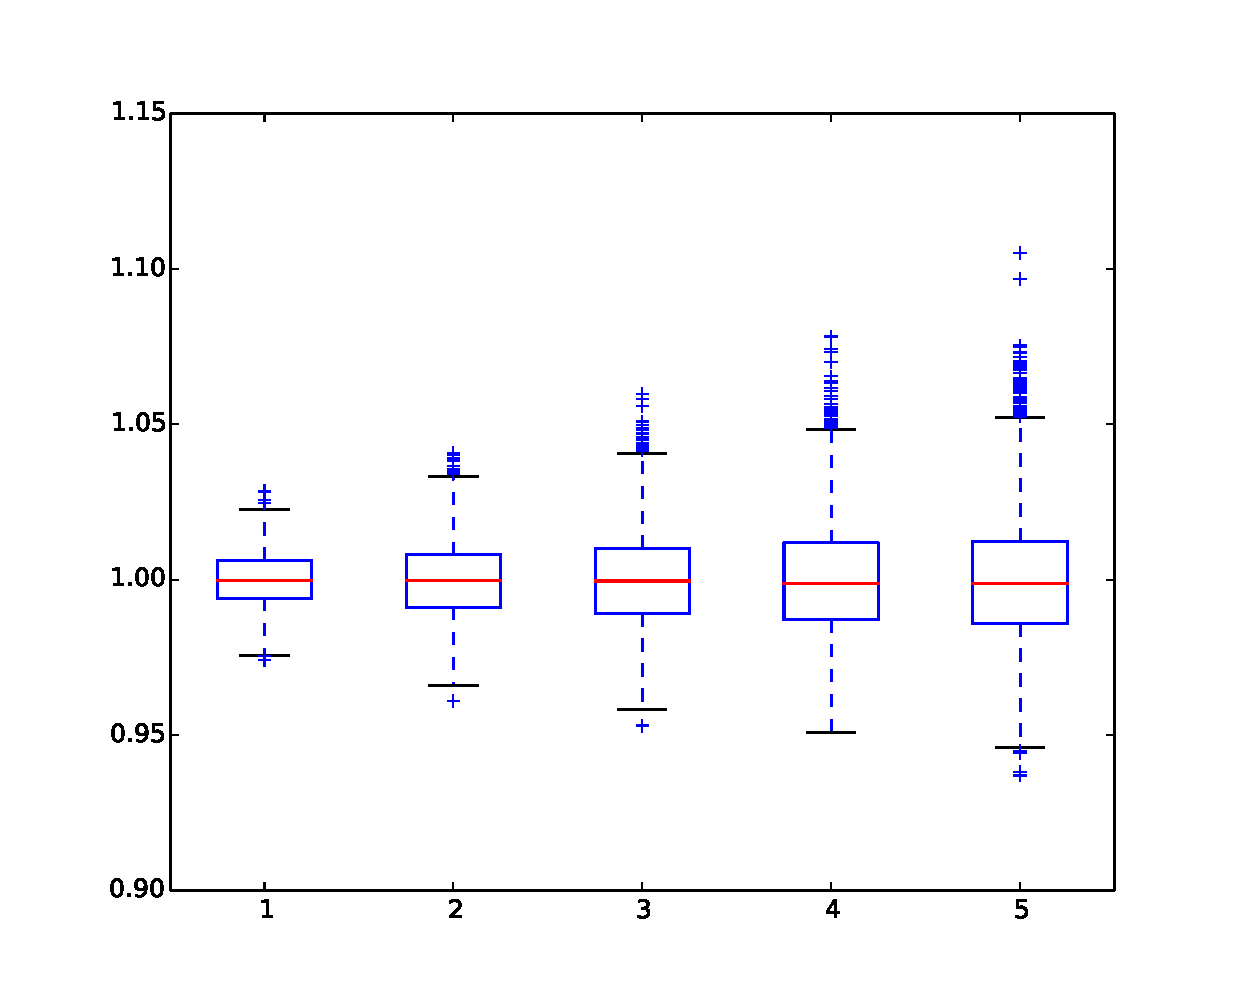
\includegraphics[scale=0.4]{full_circuit_rack_distribution.eps}
\end{figure}

\begin{itemize}
	  \item shuffle neurons on nodes pros and cons
      \item Scale of mouse brain
      \item Contains interpolation data
      \item Based on measured settings
      \item Easily adaptable, when more information are available
\end{itemize}
\subsection{Data format usability}
\begin{itemize}
      \item Synapse data format - performance vs usability
      \item Neuron data format - performance vs usability
\end{itemize}

\subsection{Parallel Efficiency}
\begin{itemize}
      \item Tested in Lugano and Juelich
      \item Strong scaling
      \item Weak scaling
\end{itemize}
\subsection{Usability for Scientists}

\begin{itemize}
      \item How to perform experiments
      \item Test different stimuli 
      \item Compare spiking activity
\end{itemize}

\end{document}
